\subsection{Finer Simulation grid}
\label{subsect: 4_finer}
As established in \autoref{subsect: 4_wall_time}, the per-CTU advantage of the latent rollout is tied to the base-case resolution: since the WaterLily solver is memory-bound, its cost per CTU grows with the grid size~\cite{Weymouth2025}, whereas a single rollout of $\mathcal{P}$ is fixed by the latent dimension $N_z = 16$ and is independent of the grid. The $256^2$ baseline used throughout this work is therefore a comparatively cheap case in which to demonstrate the gain. To investigate the effects of the hybrid loop on more expensive simulations, the reference case is re-run on a refined $512^2$ grid, keeping the Reynolds number, domain, and cylinder geometry of \autoref{tab: parameters} fixed, so that only the spatial discretisation changes. The following paragraphs will quantify how grid refinement affects the cost per CTU of the reference solver and the resulting upper bound on the achievable acceleration, together with the resolved wake itself, since a finer grid captures the secondary vortex structures of the $Re=2500$ flow more sharply, as displayed in \autoref{fig: finer_vortex_shedding}, and shifts the integrated force statistics on which the hybrid loop is assessed.


\begin{figure}[htbp]
    \centering
    \begin{subfigure}[b]{0.19\textwidth}
        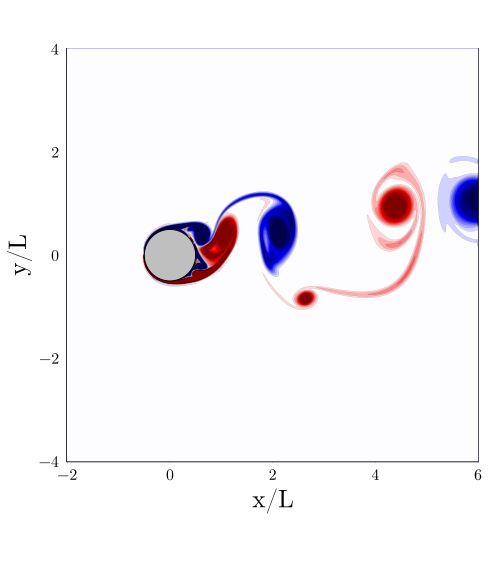
\includegraphics[width=\textwidth]{figures/Results/finer/contours/shedding_t0.1.png}
        \caption{$t^*_{n}$}
    \end{subfigure}
    \begin{subfigure}[b]{0.19\textwidth}
        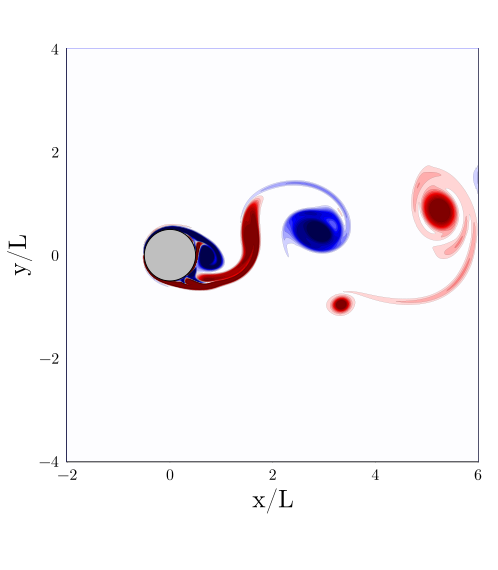
\includegraphics[width=\textwidth]{figures/Results/finer/contours/shedding_t1.1.png}
        \caption{$t^*_{n+\Delta t}$}
    \end{subfigure}
    \begin{subfigure}[b]{0.19\textwidth}
        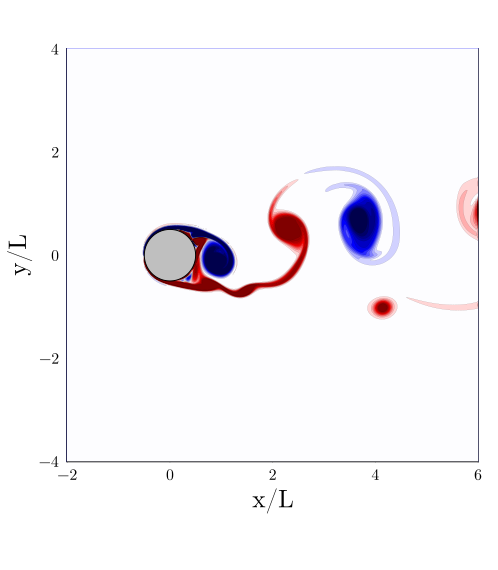
\includegraphics[width=\textwidth]{figures/Results/finer/contours/shedding_t2.1.png}
        \caption{$t^*_{n+ 2\Delta t}$}
    \end{subfigure}
    \begin{subfigure}[b]{0.19\textwidth}
        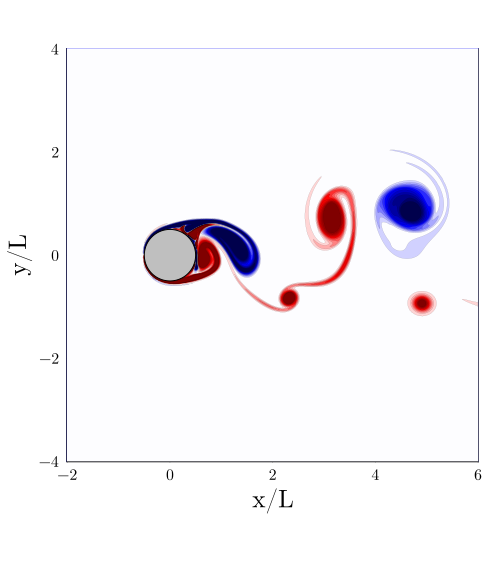
\includegraphics[width=\textwidth]{figures/Results/finer/contours/shedding_t3.1.png}
        \caption{$t^*_{n+ 3\Delta t}$}
    \end{subfigure}
    \begin{subfigure}[b]{0.19\textwidth}
        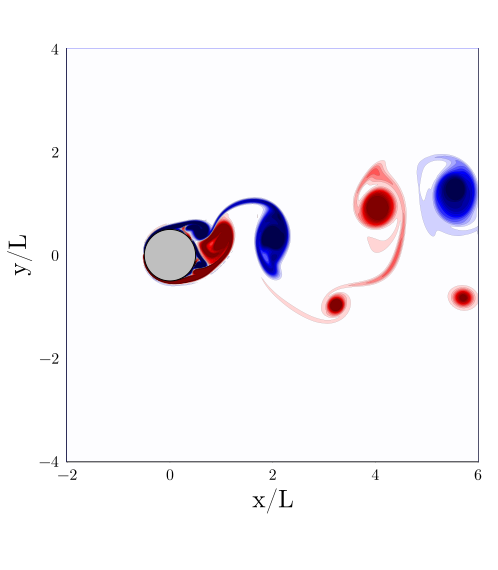
\includegraphics[width=\textwidth]{figures/Results/finer/contours/shedding_t4.2.png}
        \caption{$t^*_{n+ 4\Delta t}$}
    \end{subfigure}
    \caption{Instantaneous vorticity field $\nicefrac{\omega L}{U}$ of the finer ($512^2$) reference simulation at $Re=2500$, shown for five consecutive snapshots (left to right). Positive (red) and negative (blue) vorticity, the refined grid resolves the secondary (small-scale) structures in the wake more sharply than the $256^2$ baseline.}
    \label{fig: finer_vortex_shedding}
\end{figure}

\subsection{Wall-Time Performance}
\label{subsect: 4_finer_walltime}

Following the wall clock breakdown in \autoref{subsect: 4_wall_time}, the refined hybrid simulation is broken down into its segments, and their wall times are presented in \autoref{tab: wall_timing_hybrid_finer}. Just as in the base simulation, the initial autoencoder training consumes a very high fraction of $\mathcal{S} $'s total wall time, about $45\%$ of the total, and once the two retraining cycles are added, building and updating the networks accounts for close to $90\%$ of the $3768$~s pipeline. The CFD work, the initial data-gathering, and the two snapshot-gathering runs make up most of what remains, while the latent rollouts contribute less than $1\%$.

\begin{table}[htp]
    \centering
    \begin{tabular}{llrr}
        \toprule
        Phase & Component & Time (s) & \% of total \\
        \midrule
        initial data-gathering & -- & 190.80 & 5.06 \\
        \midrule
        \multirow{2}{*}{Train} & AE   & 1704.00 & 45.22 \\
                               & NODE &  222.00 &  5.89 \\
        \midrule
        \multirow{3}{*}{Hybrid section 1} & CFD + rollout & 1.673 & 0.04 \\
                                          & CFD + rollout & 4.057 & 0.11 \\
                                          & CFD + rollout & 4.183 & 0.11 \\
        \midrule
        \multirow{3}{*}{Retrain 1} & Gather snapshots &  95.40 &  2.53 \\
                                   & AE               & 462.00 & 12.26 \\
                                   & NODE             & 168.00 &  4.46 \\
        \midrule
        \multirow{3}{*}{Hybrid section 2} & CFD + rollout & 0.013 & 0.00 \\
                                          & CFD + rollout & 3.008 & 0.08 \\
                                          & CFD + rollout & 4.117 & 0.11 \\
        \midrule
        \multirow{3}{*}{Retrain 2} & Gather snapshots &  95.40 &  2.53 \\
                                   & AE               & 606.00 & 16.08 \\
                                   & NODE             & 204.00 &  5.41 \\
        \midrule
        Hybrid section 3 & CFD + rollout & 3.232 & 0.09 \\
        \midrule
        \textbf{Total} & & \textbf{3767.88} & \textbf{100.00} \\
        \bottomrule
    \end{tabular}
    \caption{Wall-clock breakdown of the hybrid simulation pipeline (finer $512^2$ run).}
    \label{tab: wall_timing_hybrid_finer}
\end{table}

As mentioned, the rollout cost barely changes with the grid. It is fixed by the latent dimension $N_z = 16$ and stays around $85$~ms/CTU, the same order as the base run, because it never touches the full field. The WaterLily time integrations, on the other hand, now cost $9540$~ms/CTU, against $866$~ms/CTU at $256^2$. This large cost difference between rollout and CFD is even more noticeable when inspecting the acceleration metrics, $S_\text{loop}$: 

\begin{align}
    S_\text{loop}
    &= \frac{T_\text{wall}^\text{ref}}{T_\text{wall}^\text{h, tot}}
    = \frac{954.84}{401.883} = 2.38
\end{align}

Showing that the hybrid loop uses the low-cost rollouts to its full effect, where it is able to achieve a $2.38$ speedup compared to the reference simulation. To assess the speedup of the hybrid loop compared to the training cost of the ML components of $\mathcal{P}$, the training wall time is added to the comparison in $S_\text{eff}$ with $T_\text{wall}^\text{h, training} = 3566$~s of training.

\begin{align}
    S_\text{eff}
    &= \frac{T_\text{wall}^\text{ref}}{T_\text{wall}^\text{h, tot} + T_\text{wall}^\text{h, training}}
    = \frac{954.84}{401.883 + 3366}
    = \frac{954.84}{3767.88} \approx 0.25
\end{align}

A single finer run is therefore still much slower than simply running $\mathcal{S}_\text{ref}$, because the training cost is not repaid within one simulation window. But it still performs better than the base case, which achieved an effective speedup of $0.073$, indicating that refining the grid begins to close part of the gap between the full pipeline and running the reference simulation. 

\subsection{Spatial and physical fidelity}
The finer simulation is passed to $\mathcal{P}$ without any architectural change: the architectures of $\varphi_\theta$, $\psi_\theta$ and $f_\phi$ of \autoref{sect: 4_base_hybrid} are reused as-is. The only change to the architecture is the input and output dimensions of the autoencoder, so that they can correctly pass the new, finer grid down to the latent space without dimension mismatches. An advantage of the refinement is that the decoder's
fixed cell-width smoothing now spans half the physical width, compared to the base architecture. This means that the thin separating shear layers that dominated the base-grid reconstruction error (\autoref{fig: base_velocity_comp}) are resolved by roughly twice as many cells and blurred less in physical space. Because the autoencoder can now capture fine dynamics to a much higher degree, the cost function converges much faster than before. 


\begin{figure}[htp]
    \centering
    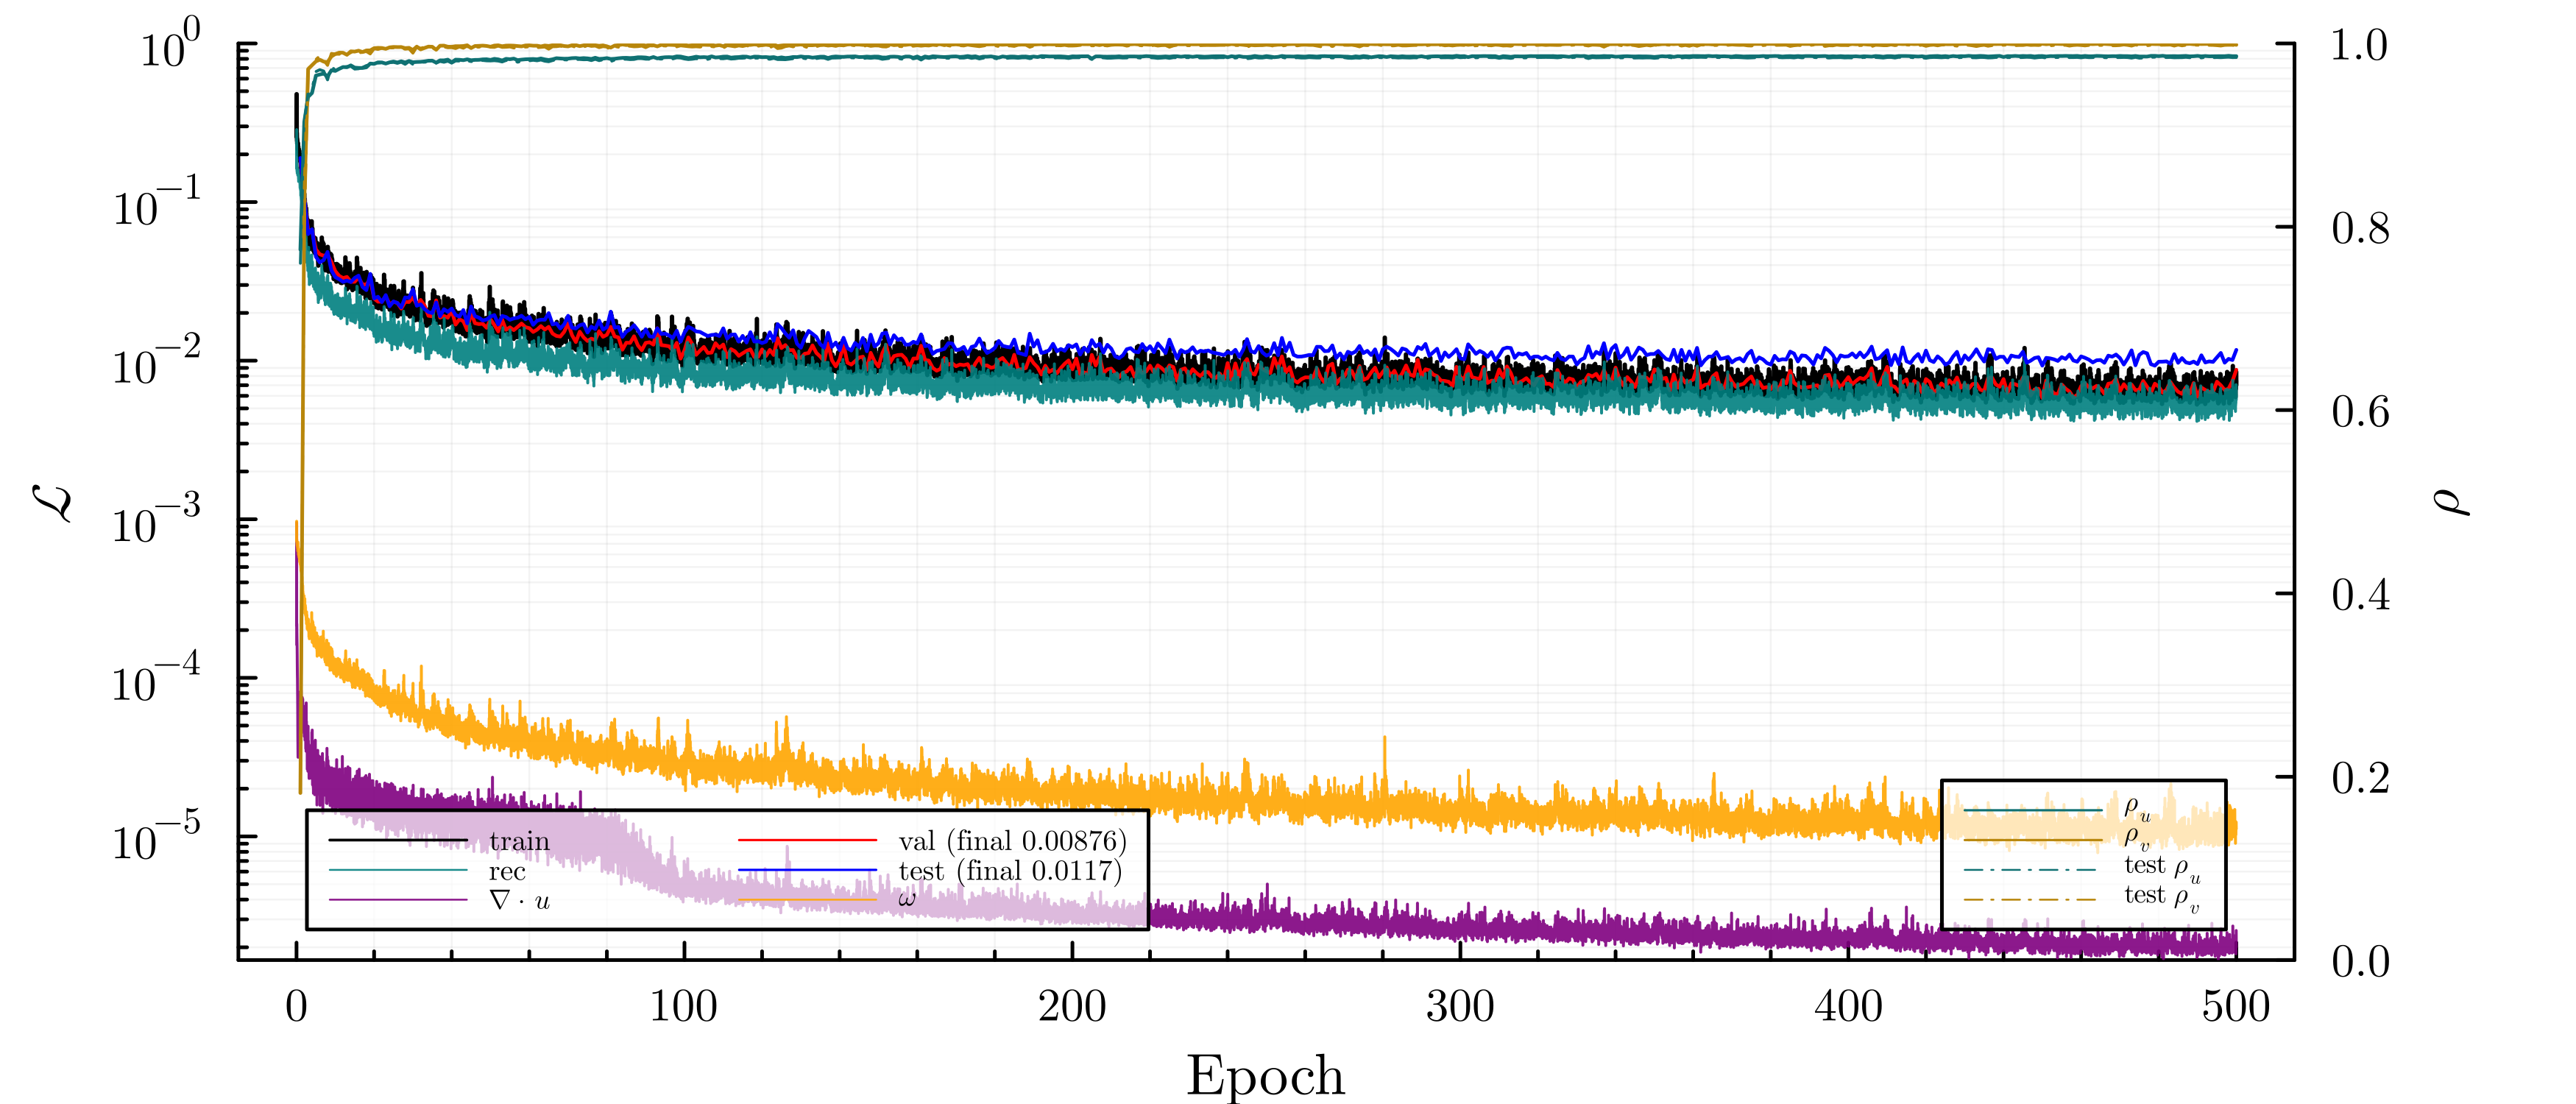
\includegraphics[width=\linewidth]{figures/Results/finer/loss_evolution.png}
    \caption{Initial training history of the autoencoder at $512^2$. Left axis ($\mathcal{L}$, logarithmic): total loss on the train, validation and test splits with the divergence ($\nabla\!\cdot\mathbf{u}$) and vorticity ($\omega$) penalties on the test split. Right axis ($CC$): reconstruction correlation coefficients $CC_u,\,CC_v$ on train and test. Validation and test losses converge to $8.6\times10^{-3}$ and $1.2\times10^{-2}$.}
    \label{fig: finer_loss}
\end{figure}

\autoref{fig: finer_loss} shows the autoencoder converging to $\mathcal{L}\approx8.6\times10^{-3}$ on the validation split and $1.2\times10^{-2}$ on the held-out test window, against $1.5\times10^{-2}$ and $3.6\times10^{-2}$ at $256^2$ (\autoref{fig: initial_training_base}).The train, validation and test curves now collapse onto one another, whereas the base case retained a test-to-validation gap of roughly a factor of two; the finer grid therefore generalises across the full simulation window rather than overfitting the initial data-gathering horizon, and $CC_u,\,CC_v$ reach unity within the first epochs.

The rapid convergence of the autoencoder shows that a large part of the training budget is spent unnecessarily: the train, validation and test losses practically collapse onto each other well before the end of the run, so there is no need to train over such a long epoch window. Since the initial autoencoder training consumes almost half of the complete integrated-workflow budget, reducing the epoch count translates directly into a higher effective speedup. If the initial autoencoder were trained for only $100$ epochs, its training cost would drop to $20\%$ of its current value. Together with a shorter update window for the retraining runs, the complete training wall time would fall to $1148.4$~s while preserving the reconstruction accuracy, since the loss is already converged at $100$ epochs. This yields an effective speedup of

\begin{align}
    S_\text{eff}
    &= \frac{T_\text{wall}^\text{ref}}{T_\text{wall}^\text{h, tot} + T_\text{wall}^\text{h, training}}
    = \frac{954.84}{401.883 + 1148.4}
    = \frac{954.84}{1550.28} \approx 0.62
\end{align}

This value shows that trimming the autoencoder schedule alone lifts $S_\text{eff}$ from $0.06$ at the base resolution to $0.62$ here, an order-of-magnitude gain that moves the integrated workflow from roughly ten times slower than the reference to within a factor of two of break-even, without touching the inference loop itself. It demonstrates that the cost of the framework is dominated by one-off training rather than by the accelerated integration: the inference loop is already cheaper than the reference, and the finer the grid, the larger that margin becomes. A single from-scratch run does not yet break even, but closing the remaining gap no longer requires a faster rollout; it requires either better use of the trained $\mathcal{P}$ across runs or overlapping training with the live simulation, together with a less strict integration monitor and switching schedule to convert the available loop speedup into actual wall-time savings.

A faithful velocity reconstruction is a key setup for the hybrid loop to accurately reproduce the loading on the cylinder. Since the force coefficients on the cylinder are calculated from the decoded velocity $\hat{\mathbf{u}}$; a reconstruction that preserves the near-body velocity, together with the divergence and vorticity penalties, feeds a more accurate pressure projection and, in turn, a more accurate integrated force. This behaviour can be seen when the force coefficients are displayed over the simulation time window in \autoref{fig: finer_forces}.

\begin{figure}[htp]
    \centering
    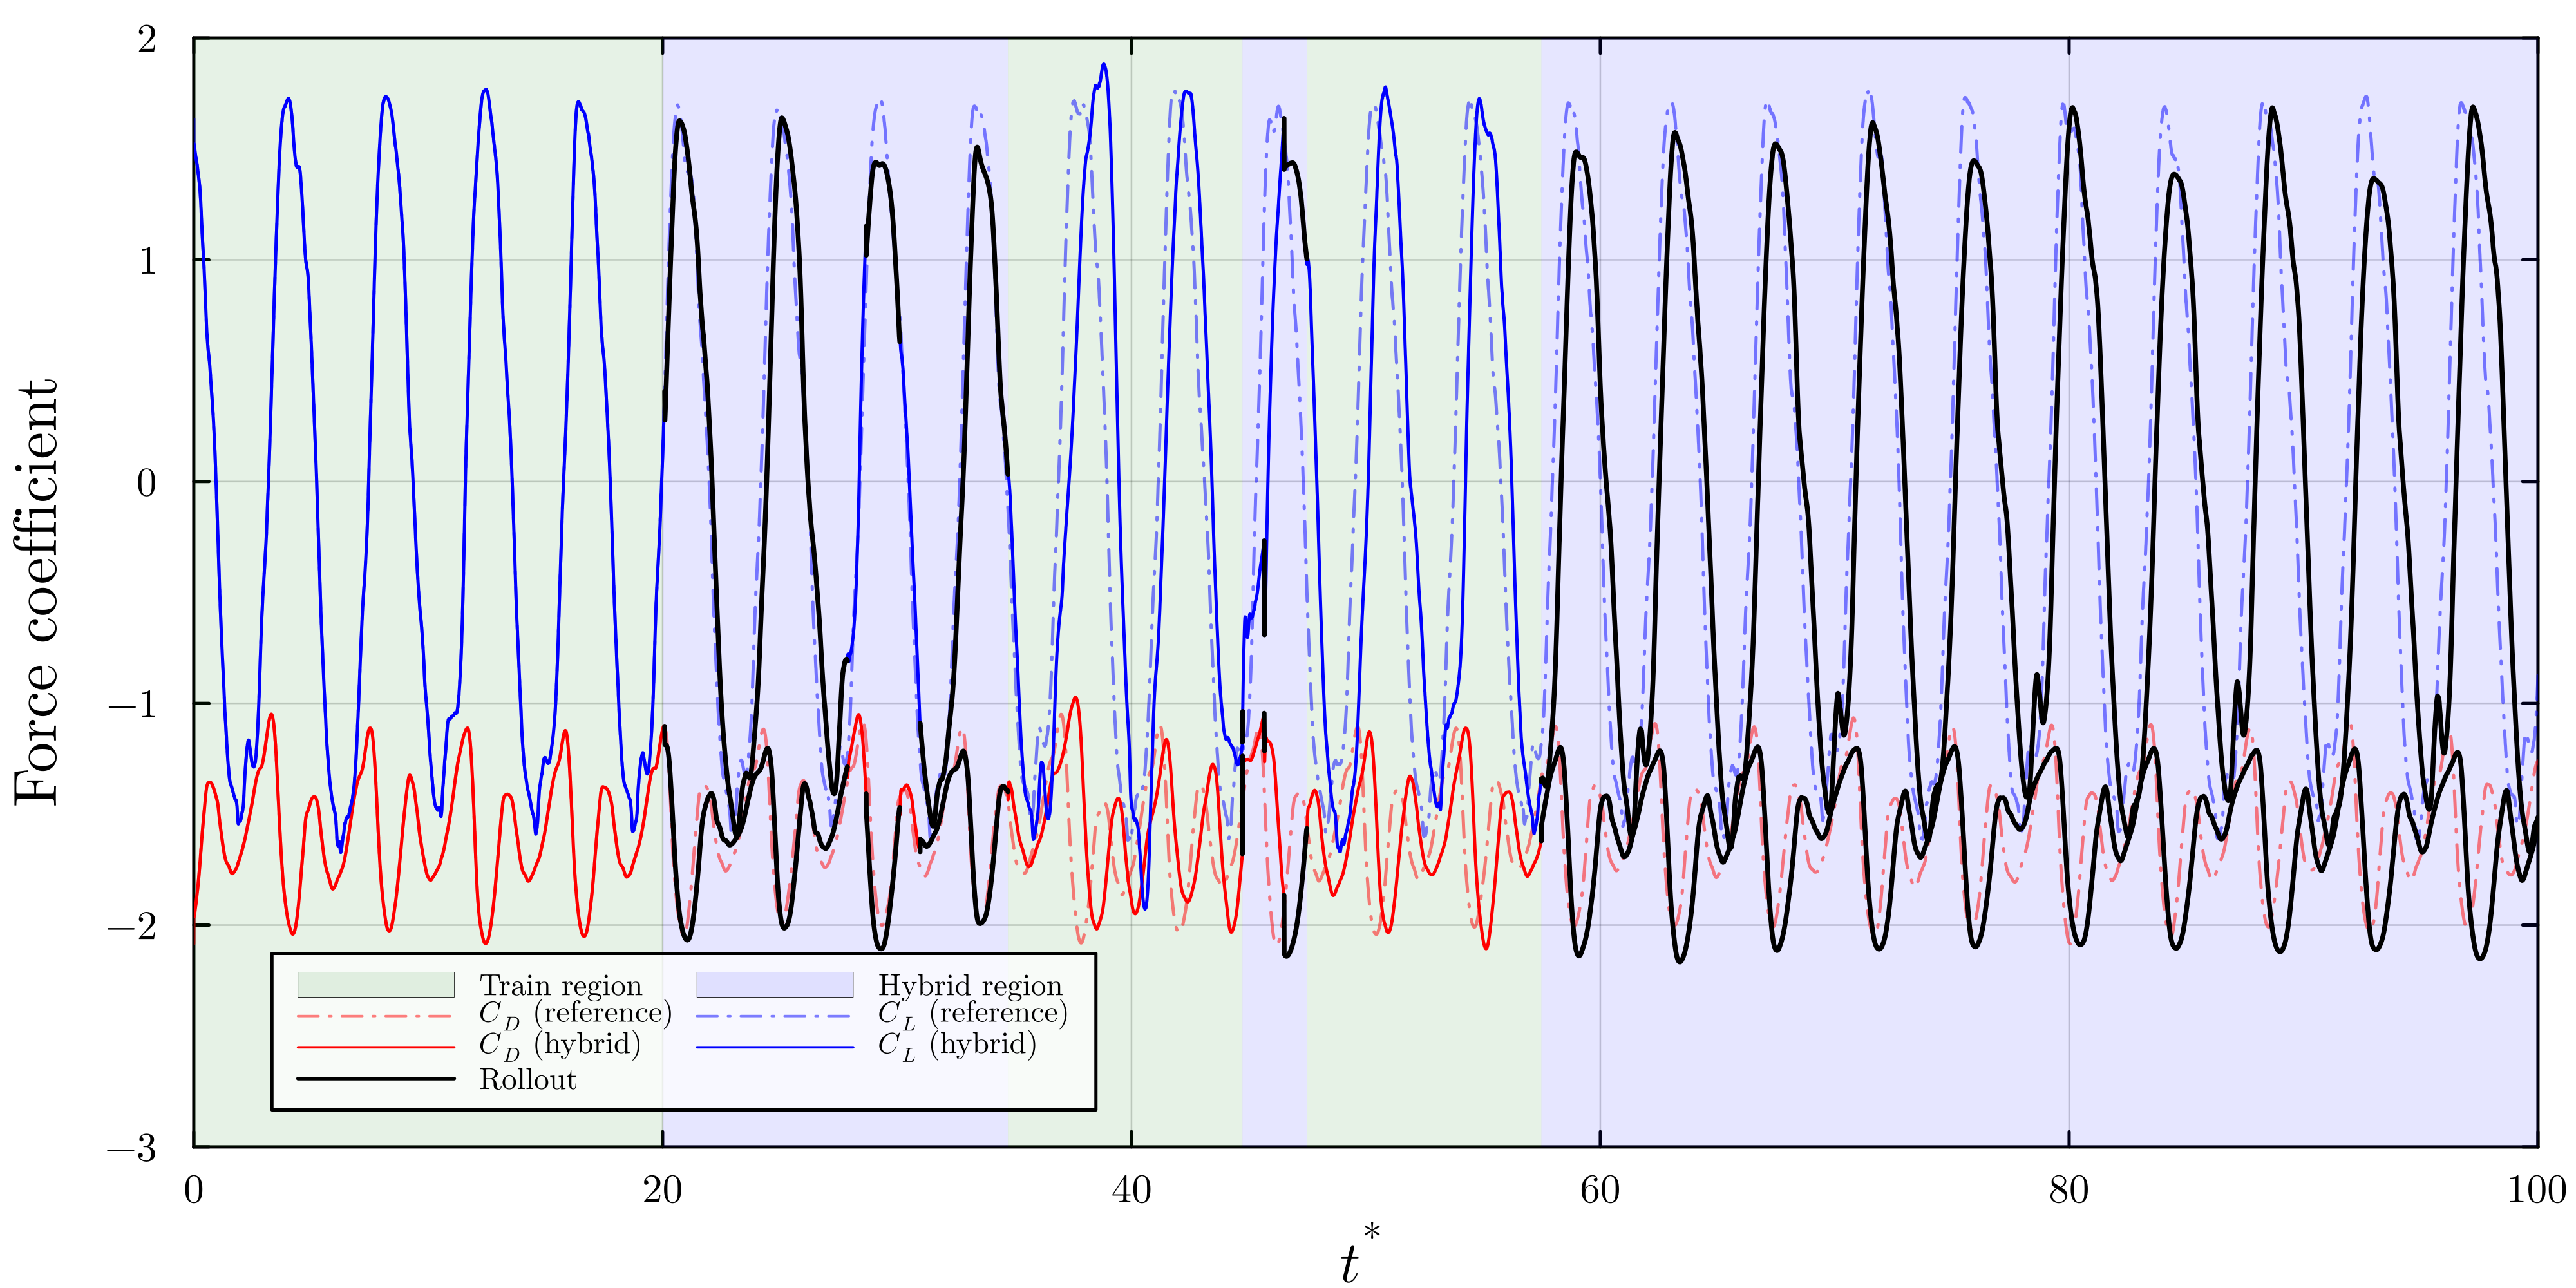
\includegraphics[width=.9\linewidth]{figures/Results/finer/forces.png}
    \caption{Lift ($C_L$) and drag ($C_D$) coefficients over $t^*$ for the finer ($512^2$) run at $Re=2500$. The hybrid loop (dashed) tracks the reference (solid) closely as an effect of the greater autoencoder performance; retraining is triggered at $t^* \approx 34.7$ and $t^* \approx 47.5$}
    \label{fig: finer_forces}
\end{figure}

\autoref{fig: finer_forces} shows that the rollouts correctly track the reference $\langle C_D \rangle$ and retain the primary shedding frequency over both the hybrid windows and the complete simulation window, with the lift preserving the shedding frequency while its fluctuation amplitude decays slightly within each rollout. This physical agreement is quantified in \autoref{tab: finer_forces}: the time-averaged drag is reproduced to within $0.64\%$ in the hybrid regions, and the time-averaged fields of \autoref{tab: finer_field} correlate with the reference at $\rho \geq 0.9966$ across the mean flow and all three Reynolds-stress
components. The only quantity that carries a visible rollout error is the lift fluctuation: the peak-weighted $C_L^\text{rms}$ error rises from $2.36\%$
over the full window to $6.83\%$ when the average is restricted to the hybrid regions. 

\begin{table}[htp]
    \centering
    \footnotesize
    \begin{subtable}[t]{0.56\textwidth}
        \centering
        \setlength{\tabcolsep}{4pt}
        \begin{tabular}{@{}lrrrr@{}}
            \toprule
            Quantity & Ref. & Hybrid & $e_\text{abs}$ & $e_\text{rel}$ [\%] \\
            \midrule
            \multicolumn{5}{l}{\textit{Full window} ($t^*\in[0,100]$)} \\
            $\langle C_D \rangle$ & $-1.57894$ & $-1.58510$ & $0.00616$ & $0.390$ \\
            $C_L^\text{rms}$      & $1.17231$  & $1.14463$  & $0.02768$ & $2.361$ \\
            \midrule
            \multicolumn{5}{l}{\textit{Hybrid regions only}} \\
            $\langle C_D \rangle$ & $-1.57201$ & $-1.58206$ & $0.01006$ & $0.640$ \\
            $C_L^\text{rms}$      & $1.16576$  & $1.08611$  & $0.07965$ & $6.832$ \\
            \bottomrule
        \end{tabular}
        \caption{Integrated force coefficients: time-mean drag
        $\langle C_D \rangle$ and r.m.s.\ lift $C_L^\text{rms}$ against the
        reference, with absolute and relative errors.}
        \label{tab: finer_forces}
    \end{subtable}
    \hfill
    \begin{subtable}[t]{0.40\textwidth}
        \centering
        \setlength{\tabcolsep}{5pt}
        \begin{tabular}{@{}lrr@{}}
            \toprule
            Quantity & $\varepsilon$ (MAE) & $\rho$ \\
            \midrule
            \multicolumn{3}{l}{\textit{Mean flow}} \\
            $\langle u \rangle$    & $0.004$ & $0.9989$ \\
            $\langle v \rangle$    & $0.004$ & $0.9970$ \\
            \midrule
            \multicolumn{3}{l}{\textit{Reynolds stresses}} \\
            $\langle u'u' \rangle$ & $0.002$ & $0.9976$ \\
            $\langle v'v' \rangle$ & $0.003$ & $0.9996$ \\
            $\langle u'v' \rangle$ & $0.001$ & $0.9966$ \\
            \bottomrule
        \end{tabular}
        \caption{Time-averaged field statistics over $\Omega$: mean absolute
        error $\varepsilon$ and spatial correlation $\rho$.}
        \label{tab: finer_field}
    \end{subtable}
    \caption{Hybrid-loop accuracy at the finer $512^2$ resolution.
    (a) integrated loading; (b) mean-flow and Reynolds-stress fields.}
    \label{tab: finer_accuracy}
\end{table}

\subsection{Latent dynamics}
\autoref{fig: finer_trajectories} shows the latent dynamics of $f_\phi$ at the finer resolution. The converged multiple-shooting fit (\autoref{fig: finer_retrain_node_ms}) reproduces all four representative components across the time windows, with $\tilde{z}$ overlaying the reference $z$ continuously through the shooting-segment boundaries of the earlier windows. The last plot of the training trajectories does show discontinuities at the segment boundaries. This mirrors the retraining imbalance identified for the base case (\autoref{subsect: 4_baseline}): since the newly augmented snapshots form a minority of the training set, so the multiple-shooting loss stays dominated by the older, well-represented dynamics and $f_\phi$ fits the newest state only weakly. 


\begin{figure}[htbp]
    \centering
    \begin{subfigure}[t]{0.48\textwidth}
        \centering
        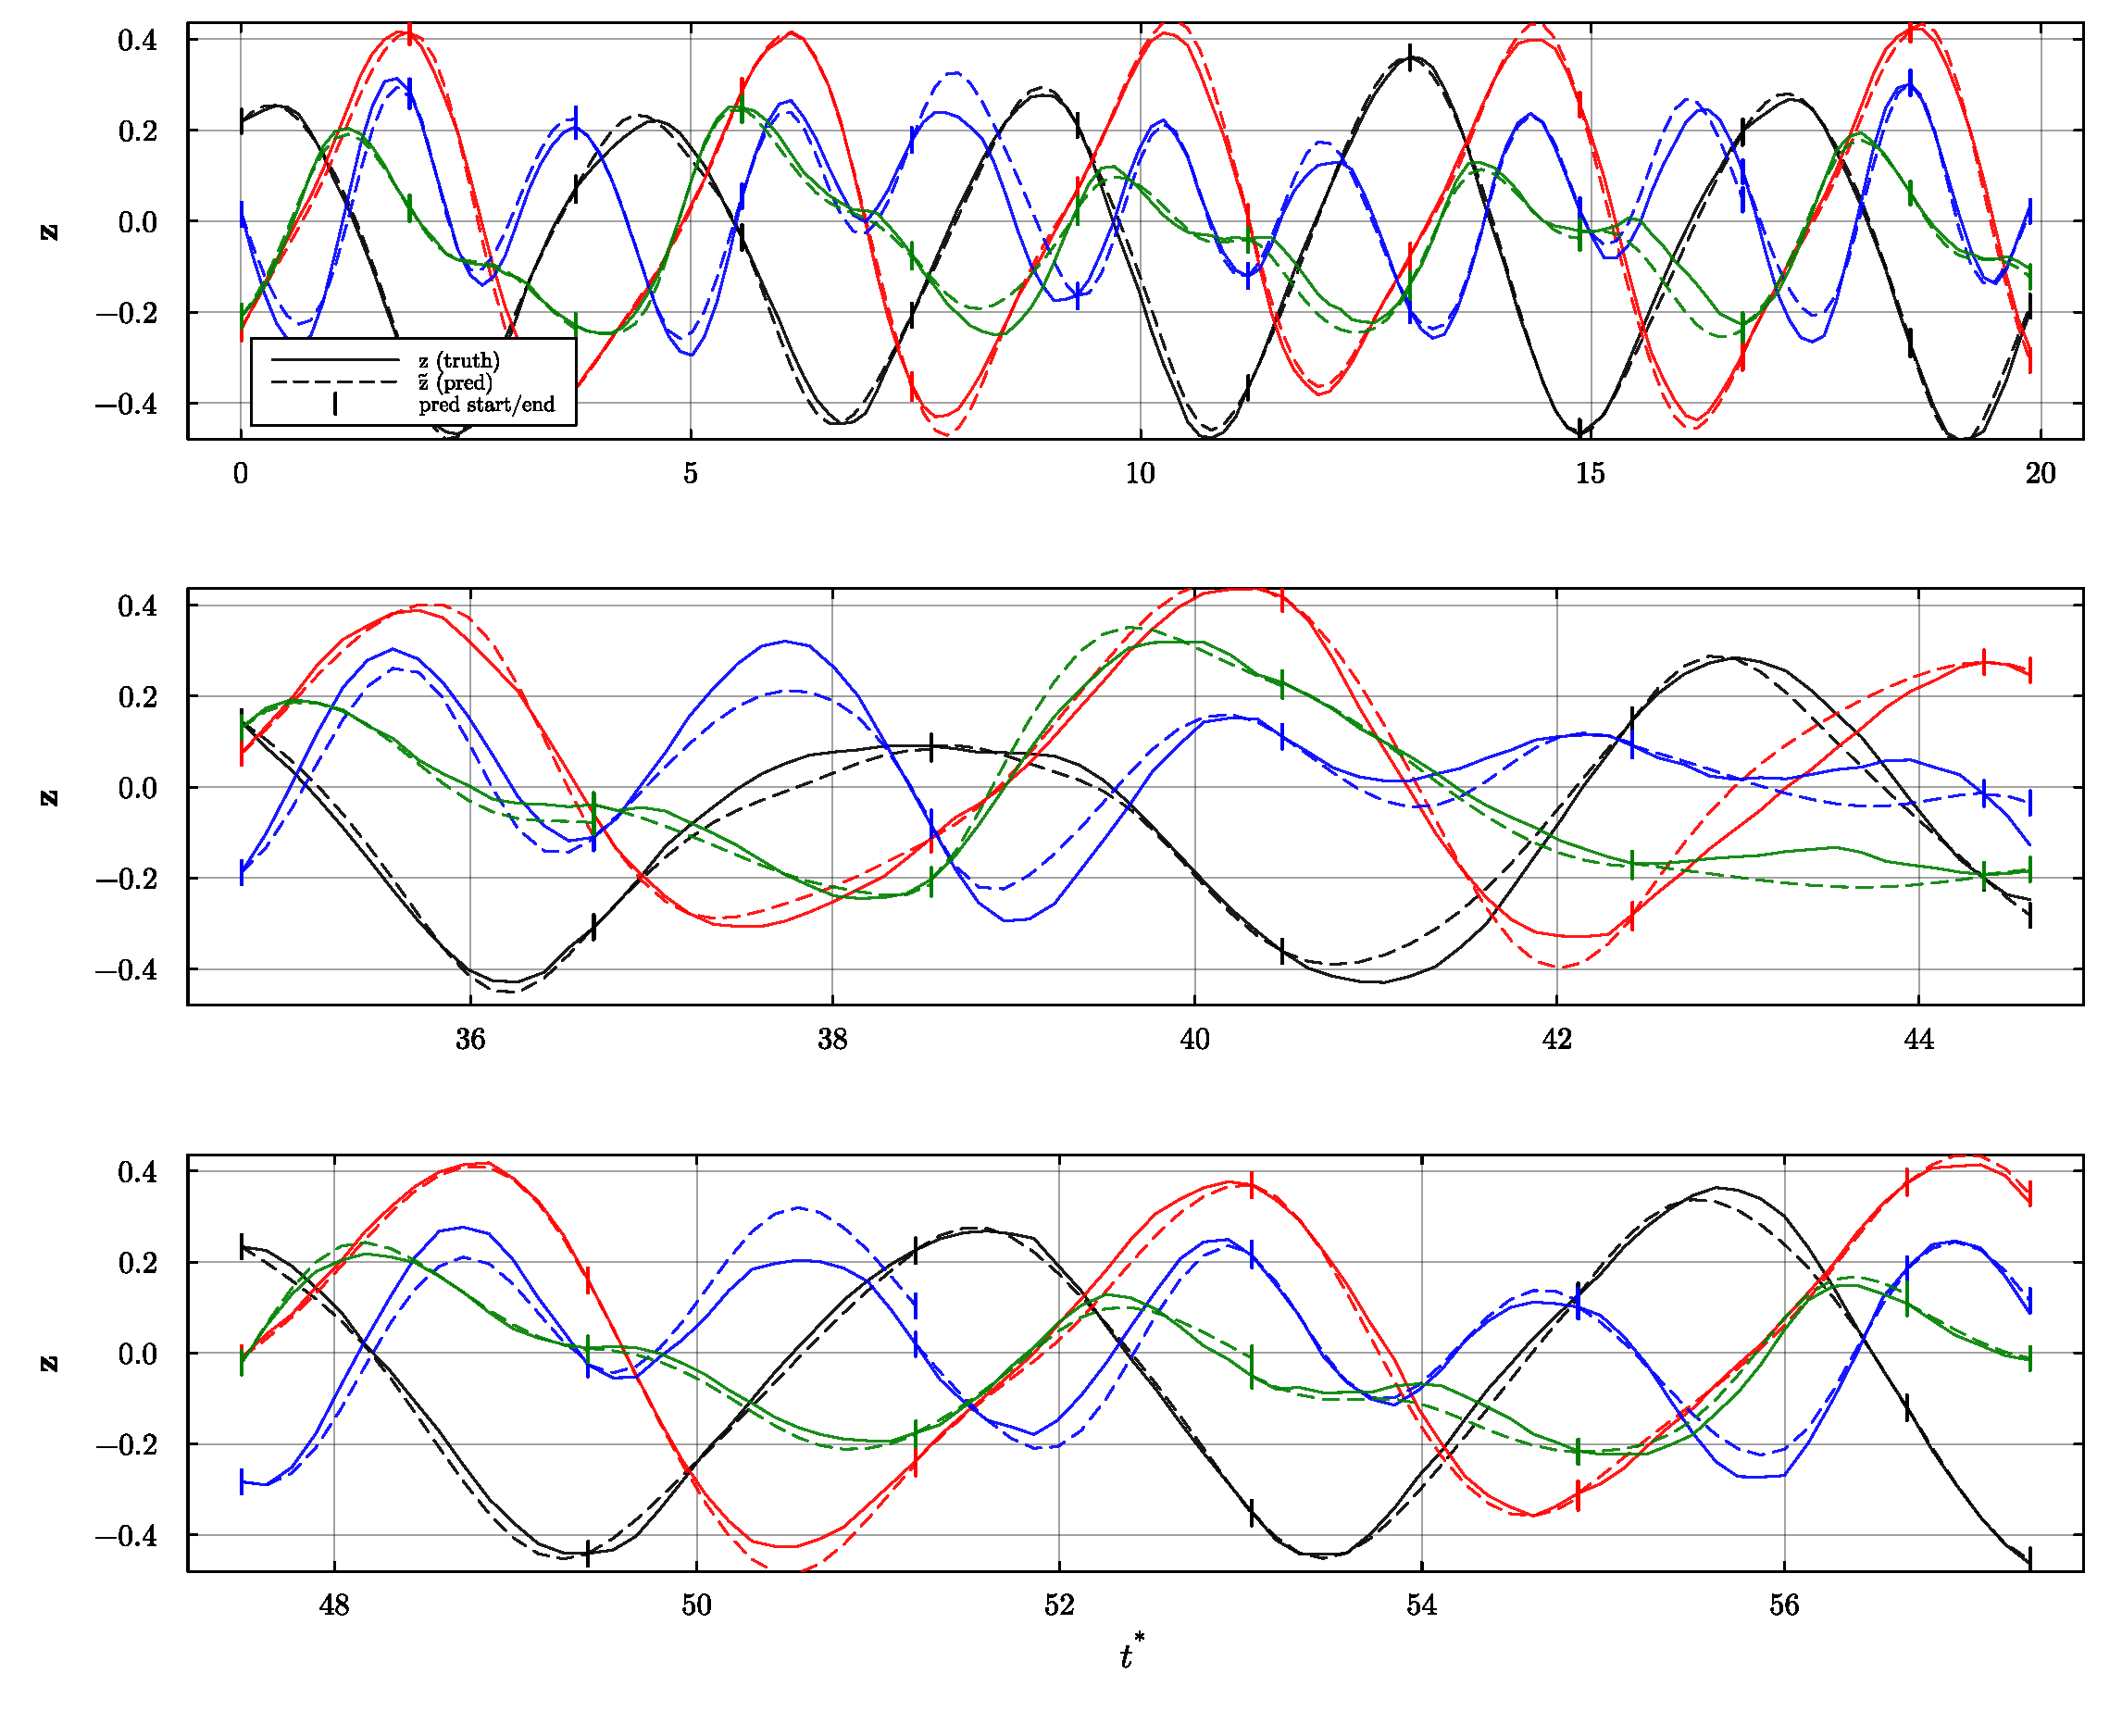
\includegraphics[width=\linewidth]{figures/Results/finer/trajectories.pdf}
    \caption{Converged multiple-shooting fit on the augmented trajectory set; markers denote shooting-segment boundaries.}
    \label{fig: finer_retrain_node_ms}
    \end{subfigure}
    \begin{subfigure}[t]{0.48\textwidth}
        \centering
        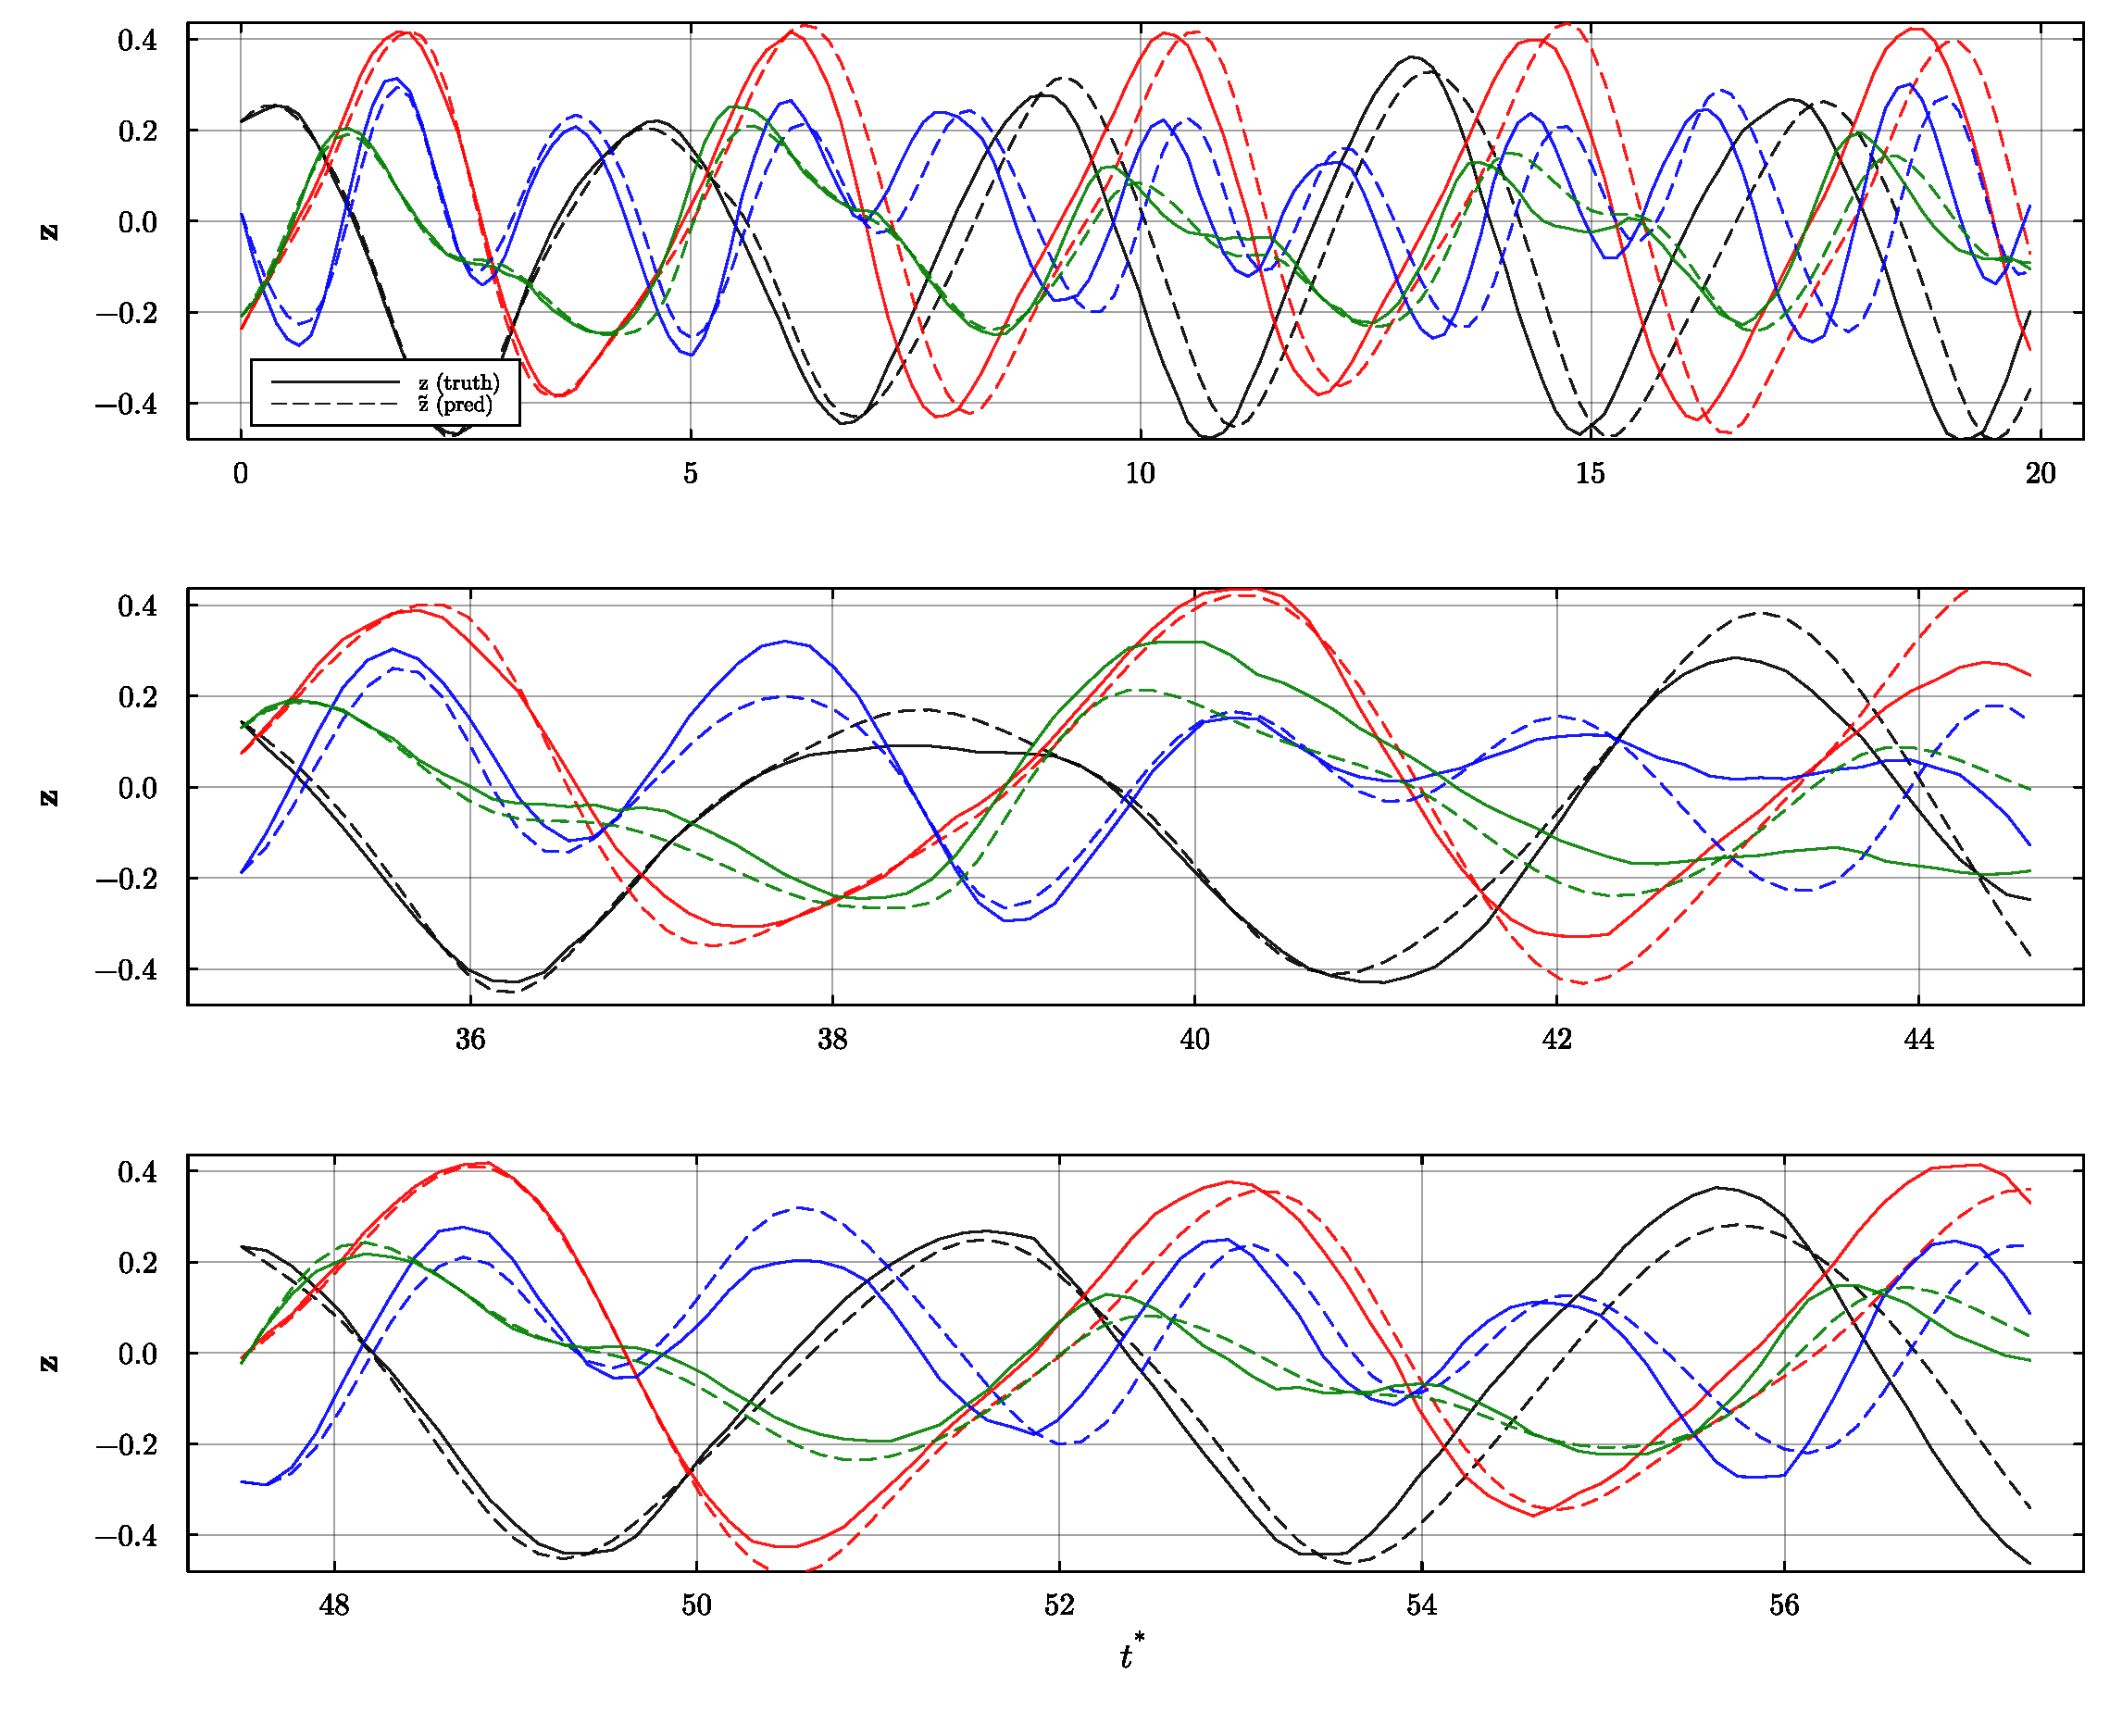
\includegraphics[width=\linewidth]{figures/Results/finer/rollout_single_shooting.pdf}
    \caption{Single rollout from $t^*=0$ across both windows after the first retraining, no segment resets.}
    \label{fig: finer_retrain_node_singleshoot}
    \end{subfigure}
    \caption{Latent dynamics of $f_\phi$ at finer grid resolution $512^2$, four representative components shown over all time windows. Reference $z$ (solid) against prediction $\tilde{z}$ (dashed). (a) Converged multiple-shooting fit on the augmented trajectory set, with segment start/end markers; (b) unaided single rollout from $t^*=0$ over the same windows.}
    \label{fig: finer_trajectories}
\end{figure}

The latent components produced by the highly accurate $\varphi_\theta$ are smooth and low in amplitude variance, showing a compact, near-periodic orbit in latent space rather than a broadly scattered cloud. Parallel to the low Re hybrid simulation discussed in \autoref{subsect: 4_re250}, this compact spread of latent vectors tightens the KNN monitor threshold $\tau$. Since the tightly clustered latent space yields small in-distribution scores and hence a small absolute $\tau$. Any divergent predictions of $\tilde{z}$ get flagged as OOD quickly and control is handed back to WaterLily, which is what caps the rollout length and forces the speedup at this resolution to come from the training budget (\autoref{subsect: 4_finer_walltime}) rather than from longer rollouts. 

The finer $512^2$ grid shows that the hybrid framework is transferable to a higher resolution without modification: the autoencoder reconstructs the velocity field more accurately and converges in a fraction of the epoch budget, the integrated drag and time-averaged fields remain near to the reference simulation, and the larger reference cost combined with the trimmable training schedule lifts the projected effective speedup by an order of magnitude over the base case. These results are promising but not complete. The $S_\text{eff}$ estimate rests on a single measured run and on the assumption that the turbulent statistics remain converged at the reduced epoch count, and the rollout length is still capped by the tight integration monitor. A dedicated study at finer resolution, covering the epoch--statistics trade-off, a measured rather than projected wall-time breakdown, and a less conservative gating schedule, could prove to be an interesting way to determine the true performance of this framework. 